\chapter{Implicit Functions}
\label{chp:implicit_functions}

\index{implicit functions}
\index{assignment operator!implicit function}

\section{Implicit Functions}

An implicit function cannot be defined as a normal function. Instead, the curve is defined as an \textit{equation} of multiple variables. It is easiest to assign a name to the entire equation, including the $=$ sign.

\begin{maplegroup}
\begin{mapleinput}
\mapleinline{active}{1d}{E := y\symbol{94}2 = x\symbol{94}3 - 2*x + 1;
}{}
\end{mapleinput}
\mapleresult
\begin{maplelatex}
\mapleinline{inert}{2d}{E := y^2 = x^3-2*x+1}{\[\displaystyle E\, := \,{y}^{2}={x}^{3}-2\,x+1\]}
\end{maplelatex}
\end{maplegroup}

\index{subs}
\index{solving equations!solve}
\index{ditto operator}

\noindent
To find points on the curve, we can substitute a value for $x$ and solve for $y$.

\begin{maplegroup}
\begin{mapleinput}
\mapleinline{active}{1d}{subs(x=2, E);
}{}
\end{mapleinput}
\mapleresult
\begin{maplelatex}
\mapleinline{inert}{2d}{y^2 = 5}{\[\displaystyle {y}^{2}=5\]}
\end{maplelatex}
\end{maplegroup}

\begin{maplegroup}
\begin{mapleinput}
\mapleinline{active}{1d}{solve(%, y);
}{}
\end{mapleinput}
\mapleresult
\begin{maplelatex}
\mapleinline{inert}{2d}{sqrt(5), -sqrt(5)}{\[\displaystyle  \sqrt{5},\,- \sqrt{5}\]}
\end{maplelatex}
\end{maplegroup}

Many implicit functions cannot be expressed as a single function $y=f(x)$. However, it may be possible to split up implicit functions into explicit functions by solving for $y$.

\index{mathematical functions!nth root@$n$\textsuperscript{th} root}

\begin{maplegroup}
\begin{mapleinput}
\mapleinline{active}{1d}{L := x\symbol{94}2 + (y - root[3](x\symbol{94}2))\symbol{94}2 = 1;
}{}
\end{mapleinput}
\mapleresult
\begin{maplelatex}
\mapleinline{inert}{2d}{L := x^2+(y-(x^2)^(1/3))^2 = 1}{\[\displaystyle L\, := \,{x}^{2}+ \left( y-\sqrt [3]{{x}^{2}} \right) ^{2}=1\]}
\end{maplelatex}
\end{maplegroup}

\marginnote[-1cm]{Here, the command \texttt{root[3]()} is equivalent to $\sqrt[3]{(~)}$.}

\begin{maplegroup}
\begin{mapleinput}
\mapleinline{active}{1d}{solve(L, y);
}{}
\end{mapleinput}
\mapleresult
\begin{maplelatex}
\mapleinline{inert}{2d}{(x^2)^(1/3)+sqrt(-x^2+1), (x^2)^(1/3)-sqrt(-x^2+1)}{\[\displaystyle \sqrt [3]{{x}^{2}}+ \sqrt{-{x}^{2}+1},\,\sqrt [3]{{x}^{2}}- \sqrt{-{x}^{2}+1}\]}
\end{maplelatex}
\end{maplegroup}

\section{Plotting Implicit Functions}

The \texttt{implicitplot()} command can be used to plot implicit functions. It requires use of the \texttt{plots} package. Unlike the normal \texttt{plot()} command, each curve that is being plotted must be in the form of an \textit{equation} of two variables, including the $=$ sign. Additionally, you must specify an interval for \textit{both} variables.
\marginnote[.6cm]{The \texttt{plots} package can be loaded using the \texttt{with()} command. This only needs to be loaded once per Maple worksheet and needs to be run each time you open a new or previously closed document.}
\index{packages!with}
\index{packages!plots}

\begin{maplegroup}
\begin{mapleinput}
\mapleinline{active}{1d}{with(plots):
}{}
\end{mapleinput}
\end{maplegroup}

\begin{maplegroup}
\begin{mapleinput}
\mapleinline{active}{1d}{implicitplot(E, x=-5..5, y=-5..5);
}{}\index{implicit functions!implicitplot!changing axes}
\end{mapleinput}
\mapleresult
\mapleplot{tutorials/figures/Implicit_Functions_and_Graphsplot2d2-eps-converted-to.pdf}
\end{maplegroup}

Most of the implicit functions used in this lab manual will produce smooth curves when plotted. See Figure \ref{fig:plotresolution} if your plot appears to have jagged edges.
\begin{marginfigure}
\index{implicit functions!implicitplot!plot resolution}
\centering
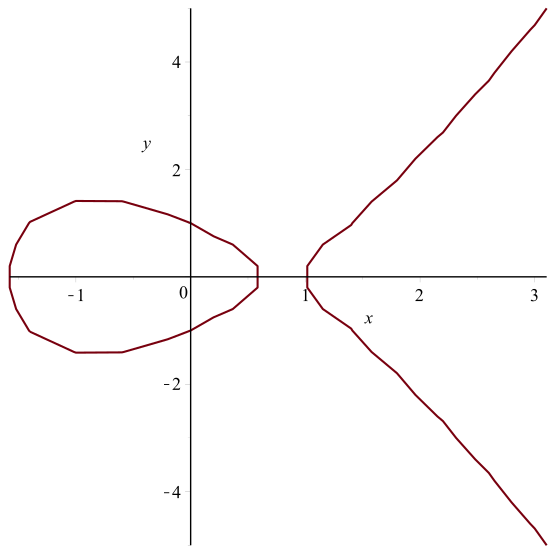
\includegraphics[scale=0.25]{tutorials/figures/Implicit_Functions_and_Graphsplot2d1-eps-converted-to.pdf}
\caption{Some versions of Maple may not produce a smooth plot of a curve, as shown here. In this case, you may need to increase the minimum number of points plotted by \texttt{implicitplot}. For example,\\
\texttt{> implicitplot(E, x=-5..5, y=-5..5, numpoints=30000);} \\
or \\
\texttt{> implicitplot(E, x=-5..5, y=-5..5, grid=[200,200]);} \\
Be careful not to choose too large of a value, otherwise the output may take a very long time to produce.}
\label{fig:plotresolution}
\end{marginfigure}

\index{implicit functions!implicitplot!filledregions}
\begin{maplegroup}
\begin{mapleinput}
\mapleinline{active}{1d}{implicitplot(L, x=-1.2..1.2, y=-1.2..1.8, coloring = ["red","blue"], filledregions=true);
}{}
\index{implicit functions!implicitplot!colour}
\end{mapleinput}
\mapleresult
\mapleplot{tutorials/figures/Implicit_Functions_and_Graphsplot2d3-eps-converted-to.pdf}
\end{maplegroup}

\section{Implicit Differentiation}

We need to use the \texttt{implicitdiff()} command to find the derivative of an implicit function. It is easiest to first assign a name to the equation.

\begin{maplegroup}
\begin{mapleinput}
\mapleinline{active}{1d}{E := y = x\symbol{94}2 + x;
}{}
\end{mapleinput}
\mapleresult
\begin{maplelatex}
\mapleinline{inert}{2d}{E := y = x^2+x}{\[\displaystyle E\, := \,y={x}^{2}+x\]}
\end{maplelatex}
\end{maplegroup}

\index{assignment operator!implicit function}
\index{packages!with}
\index{packages!plots}
\index{implicit functions!implicitplot!changing axes}
\index{implicit functions!implicitplot!plot resolution}
\index{implicit functions!implicitdiff}

\begin{maplegroup}
\begin{mapleinput}
\mapleinline{active}{1d}{with(plots):
}{}
\end{mapleinput}
\end{maplegroup}

\begin{maplegroup}
\begin{mapleinput}
\mapleinline{active}{1d}{implicitplot(E, x=-5..5, y=-5..5);
}{}
\end{mapleinput}
\mapleresult
\mapleplot{tutorials/figures/Implicit_Functions_and_Differentiationplot2d1-eps-converted-to.pdf}
\end{maplegroup}

\begin{maplegroup}
\begin{mapleinput}
\mapleinline{active}{1d}{dydx := implicitdiff(E, y, x);
}{}
\end{mapleinput}
\mapleresult
\begin{maplelatex}
\mapleinline{inert}{2d}{dydx := 2*x+1}{\[\displaystyle {\it dydx}\, := \,2\,x+1\]}
\end{maplelatex}
\end{maplegroup}

The order in which you list the variables matters; the first variable is treated as the dependent variable and the second variable is treated as the independent variable.
\marginnote{To find $dy/dx$, you must use \texttt{implicitdiff(E,y,x)} and to find $dx/dy$, you  must use \texttt{implicitdiff(E,x,y)}.}

\begin{maplegroup}
\begin{mapleinput}
\mapleinline{active}{1d}{dxdy := implicitdiff(E, x, y);
}{}
\end{mapleinput}
\mapleresult
\begin{maplelatex}
\mapleinline{inert}{2d}{dxdy := 1/(2*x+1)}{\[\displaystyle {\it dxdy}\, := \, \frac{1}{2\,x+1}\]}
\end{maplelatex}
\end{maplegroup}

When trying to find the slope of a tangent line at a point on an implicit curve, it helps to plot the curve first.

\index{mathematical functions!nth root@$n$\textsuperscript{th} root}

\begin{maplegroup}
\begin{mapleinput}
\mapleinline{active}{1d}{L := x\symbol{94}2 + (y - root[3](x\symbol{94}2))\symbol{94}2 = 1;
}{}
\end{mapleinput}
\mapleresult
\begin{maplelatex}
\mapleinline{inert}{2d}{L := x^2+(y-(x^2)^(1/3))^2 = 1}{\[\displaystyle L\, := \,{x}^{2}+ \left( y-\sqrt [3]{{x}^{2}} \right) ^{2}=1\]}
\end{maplelatex}
\end{maplegroup}

\begin{maplegroup}
\begin{mapleinput}
\mapleinline{active}{1d}{implicitplot(L, x=-1.2..1.2, y=-1.2..1.8);
}{}
\end{mapleinput}
\mapleresult
\mapleplot{tutorials/figures/Implicit_Functions_and_Differentiationplot2d2-eps-converted-to.pdf}
\end{maplegroup}

\noindent
To find the points on the curve at a specific $x$ value, you must first substitute the value and then solve for the $y$-coordinates.

\index{subs}
\index{solving equations!fsolve}

\begin{maplegroup}
\begin{mapleinput}
\mapleinline{active}{1d}{subs(x=0.5, L); yCoords := fsolve(%, y);
}{}
\end{mapleinput}
\mapleresult
\begin{maplelatex}
\mapleinline{inert}{2d}{.25+(y-.6299605249)^2 = 1}{\[\displaystyle  0.25+ \left( y- 0.6299605249 \right) ^{2}=1\]}
\end{maplelatex}
\marginnote{Notice that a list of two $y$-coordinates is assigned to a single name here. You could assign the individual values to unique names.}
\begin{maplelatex}
\mapleinline{inert}{2d}{yCoords := 1.495985929, -.2360648789}{\[\displaystyle {\it yCoords}\, := \, 1.495985929,\,- 0.2360648789\]}
\end{maplelatex}
\end{maplegroup}

\noindent
Then you can find the slopes of the tangent lines by computing the derivative with \texttt{implicitdiff()} and substituting the $x$ and $y$ values for each point.

\begin{maplegroup}
\begin{mapleinput}
\mapleinline{active}{1d}{dydx := implicitdiff(L, y, x);
}{}
\end{mapleinput}
\mapleresult
\begin{maplelatex}
\mapleinline{inert}{2d}{dydx := x*(-3*(x^2)^(2/3)-2*(x^2)^(1/3)+2*y)/(3(x^2)^(2/3)*y-x^2)}{\[\displaystyle {\it dydx}\, := \,{\frac {x \left( -3\, \left( {x}^{2} \right) ^{2/3}-2\,\sqrt [3]{{x}^{2}}+2\,y \right) }{ 3\left(y\left( {x}^{2} \right) ^{2/3}-{x}^{2}\right)}}\]}
\end{maplelatex}
\end{maplegroup}

\begin{maplegroup}
\begin{mapleinput}
\mapleinline{active}{1d}{subs(x=0.5, y=yCoords[1], dydx);
}{}
\end{mapleinput}
\mapleresult
\begin{maplelatex}
\mapleinline{inert}{2d}{.2625970976}{\[\displaystyle  0.2625970976\]}
\end{maplelatex}
\end{maplegroup}

\marginnote{\texttt{yCoords} is the name that both values are assigned to. To refer to an individual value, we use the index of the desired value in square brackets after the name \texttt{yCoords}.}

\begin{maplegroup}
\begin{mapleinput}
\mapleinline{active}{1d}{subs(x=0.5, y=yCoords[2], dydx);
}{}
\end{mapleinput}
\mapleresult
\begin{maplelatex}
\mapleinline{inert}{2d}{1.417297636}{\[\displaystyle  1.417297636\]}
\end{maplelatex}
\end{maplegroup}

\section{Applications of Implicit Differentiation}

In these examples, we will make use of the \texttt{implicitdiff()} and \texttt{implicitplot()} commands.

\subsection{Finding the Equation of a Tangent Line}
\label{subsec:implicittanline}

\index{lines!tangent line!implicit function}

In this example, we will find the equations of the tangent lines to the circle of radius $4$, centred at the point $(1,1)$, where $x=3$. 
\marginnote{The equation of a circle that is centred at the point $(a,b)$ and has radius $r$ is
\[ (x-a)^2+(y-b)^2=r^2. \]}

\begin{maplegroup}
\begin{mapleinput}
\mapleinline{active}{1d}{circle := (x-1)\symbol{94}2 + (y-1)\symbol{94}2 = 16;
}{}
\end{mapleinput}
\mapleresult
\begin{maplelatex}
\mapleinline{inert}{2d}{circle := (x-1)^2+(y-1)^2 = 16}{\[\displaystyle {\it circle}\, := \,{(x-1)}^{2}+{(y-1)}^{2}=16\]}
\end{maplelatex}
\end{maplegroup}

We need to find the $y$-coordinates by substituting $x=3$ and solving for $y$.

\begin{maplegroup}
\begin{mapleinput}
\mapleinline{active}{1d}{subs(x=3, circle); yCoords:=solve(%, y);
}{}
\end{mapleinput}
\mapleresult
\begin{maplelatex}
\mapleinline{inert}{2d}{4+(y-1)^2 = 16}{\[\displaystyle 4+(y-1)^2 = 16\]}
\end{maplelatex}
\mapleresult
\begin{maplelatex}
\mapleinline{inert}{2d}{yCoords := 1+2\sqrt{3}, 1-2\sqrt(3)}{\[\displaystyle {\it yCoords}\, := \, 1+2\sqrt{3},\,1-2\sqrt{3}\]}
\end{maplelatex}
\end{maplegroup}

The derivative $\tfrac{dy}{dx}$ can be found using \texttt{implicitdiff()}. Then, by substituting the two points, we can find the slopes of both tangent lines.

\index{implicit functions!implicitdiff}
\index{subs}

\begin{maplegroup}
\begin{mapleinput}
\mapleinline{active}{1d}{dydx := implicitdiff(circle, y, x);
}{}
\end{mapleinput}
\mapleresult
\begin{maplelatex}
\mapleinline{inert}{2d}{dydx := -(x-1)/(y-1)}{\[\displaystyle {\it dydx}\, := \,-{\frac {x-1}{y-1}}\]}
\end{maplelatex}
\end{maplegroup}

\marginnote{Make sure that you choose different names when assigning values. We will need both slopes later.}

\begin{maplegroup}
\begin{mapleinput}
\mapleinline{active}{1d}{m1 := subs(x=3, y=yCoords[1], dydx);
}{}
\end{mapleinput}
\mapleresult
\begin{maplelatex}
\mapleinline{inert}{2d}{m1 := -\frac{1}{3}\sqrt{3}}{\[\displaystyle {\it m1}\, := \,-\frac{1}{3}\sqrt{3}\]}
\end{maplelatex}
\end{maplegroup}

\begin{maplegroup}
\begin{mapleinput}
\mapleinline{active}{1d}{m2 := subs(x=3, y=yCoords[2], dydx);
}{}
\end{mapleinput}
\mapleresult
\begin{maplelatex}
\mapleinline{inert}{2d}{m2 :=\frac{1}{3}\sqrt{3}}{\[\displaystyle {\it m2}\, := \,\frac{1}{3}\sqrt{3}\]}
\end{maplelatex}
\end{maplegroup}
\clearpage
Thinking ahead, in order to plot both lines using \texttt{implicitplot()}, they will need to be defined as \textit{equations}.

\index{subs}

\begin{maplegroup}
\begin{mapleinput}
\mapleinline{active}{1d}{line1 := y = m1*(x-3) + yCoords[1];expand(\%);
}{}
\end{mapleinput}
\mapleresult
\begin{maplelatex}
\mapleinline{inert}{2d}{line1 := y = -\frac{1}{3}\sqrt{3}(x-3)+1+2\sqrt{3}}{\[\displaystyle {\it line1}\, := \,y=-\frac{1}{3}\sqrt{3}(x-3)+1+2\sqrt{3}\]}
\end{maplelatex}
\begin{maplelatex}
\mapleinline{inert}{2d}{y = -\frac{1}{3}\sqrt{3}x+3\sqrt{3}+1}{\[\displaystyle  y=-\frac{1}{3}\sqrt{3}x+3\sqrt{3}+1\]}
\end{maplelatex}
\end{maplegroup}

\marginnote{Both \texttt{line1} and \texttt{line2} are defined with the inclusion of $y=$, making them equations that \texttt{implicitplot()} can plot.}

\begin{maplegroup}
\begin{mapleinput}
\mapleinline{active}{1d}{line2 := y = m2*(x-3) + yCoords[2];expand(\%);
}{}
\end{mapleinput}
\mapleresult
\begin{maplelatex}
\mapleinline{inert}{2d}{line2 := y = \frac{1}{3}\sqrt{3}(x-3)+1-2\sqrt{3}}{\[\displaystyle {\it line2}\, := \,y=\frac{1}{3}\sqrt{3}(x-3)+1-2\sqrt{3}\]}
\end{maplelatex}
\begin{maplelatex}
\mapleinline{inert}{2d}{y = \frac{1}{3}\sqrt{3}x-3\sqrt{3}+1}{\[\displaystyle  y=\frac{1}{3}\sqrt{3}x-3\sqrt{3}+1\]}
\end{maplelatex}
\end{maplegroup}

We can now plot the circle and the two lines together.

\index{packages!plots}
\index{implicit functions!implicitplot!scaling}
\index{implicit functions!implicitplot!multiple curves}
\index{implicit functions!implicitplot!changing axes}
\index{implicit functions!implicitplot!plot resolution}
\index{implicit functions!implicitplot!colour}

\begin{maplegroup}
\begin{mapleinput}
\mapleinline{active}{1d}{with(plots):
}{}
\end{mapleinput}
\end{maplegroup}

\begin{maplegroup}
\begin{mapleinput}
\mapleinline{active}{1d}{implicitplot([circle, line1, line2], x=-8..8, y=-8..8, colour=[red,blue,green], scaling=constrained);
}{}
\end{mapleinput}
\mapleresult
\mapleplot{tutorials/figures/ImplicitTangentCircle.eps}
\end{maplegroup}

\marginnote[-4cm]{Using the \texttt{scaling=constrained} parameter will produce a proper circle in your worksheet. The graph can also be scaled without using the \texttt{scaling=constrained} parameter; simply click on the graph and then click on the \includegraphics[scale=0.5]{tutorials/figures/1-1.png} button in the plot toolbar at the top of the page.}

\subsection{Orthogonal Curves}
\label{subsec:orthocurves}

In this example, we will show that the curves $x^2 - y^2 = 8$ and $-xy =~3$ are always perpendicular (orthogonal) at their intersection points.

\begin{maplegroup}
\begin{mapleinput}
\mapleinline{active}{1d}{curve1 := x\symbol{94}2 - y\symbol{94}2 = 8;
}{}
\end{mapleinput}
\mapleresult
\begin{maplelatex}
\mapleinline{inert}{2d}{curve1 := x^2-y^2 = 8}{\[\displaystyle {\it curve1}\, := \,{x}^{2}-{y}^{2}=8\]}
\end{maplelatex}
\end{maplegroup}


\begin{maplegroup}
\begin{mapleinput}
\mapleinline{active}{1d}{curve2 := -x*y = 3;
}{}
\end{mapleinput}
\mapleresult
\begin{maplelatex}
\mapleinline{inert}{2d}{curve2 := -x*y = 23}{\[\displaystyle {\it curve2}\, := \,-xy=3\]}
\end{maplelatex}
\end{maplegroup}

\begin{maplegroup}
\begin{mapleinput}
\mapleinline{active}{1d}{with(plots):
}{}
\end{mapleinput}
\end{maplegroup}

\marginnote[-1.5cm]{We must include multiplication between $x$ and $y$ here, otherwise Maple will think we want to use a variable called $xy$.}

\begin{maplegroup}
\begin{mapleinput}
\mapleinline{active}{1d}{implicitplot([curve1, curve2], x=-5..5, y=-5..5, colour=[red, blue], scaling=constrained);
}{}
\end{mapleinput}
\mapleresult
\mapleplot{tutorials/figures/OrthogonalCurves2.eps}
\end{maplegroup}

\marginnote[-1cm]{Using the \texttt{scaling=constrained} parameter will preserve right angles in your worksheet.}

From the graphs of these two curves, it appears that their intersections are perpendicular. This can be proven by showing that the derivative of one curve is equal to the negative reciprocal of the other, or that they multiply to equal $-1$.

The intersection points can be found by solving a system of equations.

\index{solving equations!intersection points}
\index{implicit functions!implicitdiff}
\index{subs}

\marginnote[0.5cm]{Using the option \texttt{explicit=true} here will avoid the use of \textit{RootOf} in the output. Optionally, using \texttt{fsolve()} may be preferable. Points involving $I$ are imaginary points and should not be considered.}

\begin{maplegroup}
\begin{mapleinput}
\mapleinline{active}{1d}{solve(\{curve1, curve2\}, \{x, y\}, explicit = true);
}{}
\end{mapleinput}
\mapleresult
\begin{maplelatex}
\mapleinline{inert}{2d}{{x = -3, y = 1}, {x = 3, y = -1}, {x = I, y = 3*I}, {x = -I, y = -3*I}}{\[\displaystyle  \left\{ x=-3,y=1 \right\} ,\, \left\{ x=3,y=-1 \right\} ,\, \left\{ x=I,y=3\,I \right\} ,\, \left\{ x= -I,y=-3\,I \right\} \]}
\end{maplelatex}
\end{maplegroup}

The derivatives of both curves can be found implicitly using the \texttt{implicitdiff()} command.

\begin{maplegroup}
\begin{mapleinput}
\mapleinline{active}{1d}{dydx1 := implicitdiff(curve1, y, x);
}{}
\end{mapleinput}
\mapleresult
\begin{maplelatex}
\mapleinline{inert}{2d}{dydx1 := x/y}{\[\displaystyle {\it dydx1}\, := \,{\frac {x}{y}}\]}
\end{maplelatex}
\end{maplegroup}

\begin{maplegroup}
\begin{mapleinput}
\mapleinline{active}{1d}{dydx2 := implicitdiff(curve2, y, x);
}{}
\end{mapleinput}
\mapleresult
\begin{maplelatex}
\mapleinline{inert}{2d}{dydx2 := -y/x}{\[\displaystyle {\it dydx2}\, := \,-{\frac {y}{x}}\]}
\end{maplelatex}
\end{maplegroup}

To show that the slopes are negative reciprocals, a point can be substituted into the two derivatives.

\begin{maplegroup}
\begin{mapleinput}
\mapleinline{active}{1d}{subs(x=-3, y=1, dydx1);
}{}
\end{mapleinput}
\mapleresult
\begin{maplelatex}
\mapleinline{inert}{2d}{-3}{\[\displaystyle -3\]}
\end{maplelatex}
\begin{mapleinput}
\mapleinline{active}{1d}{subs(x=-3, y=1, dydx2);
}{}
\end{mapleinput}
\mapleresult
\begin{maplelatex}
\mapleinline{inert}{2d}{\frac{1}{3}}{\[\displaystyle \frac{1}{3}\]}
\end{maplelatex}
\end{maplegroup}

Alternatively, it can be shown that the derivatives are negative reciprocals of each other in general.

\marginnote{Recall that two slopes $m_1$ and $m_2$ are perpendicular if $m_1 m_2 = -1$.}

\begin{maplegroup}
\begin{mapleinput}
\mapleinline{active}{1d}{dydx1*dydx2;
}{}
\end{mapleinput}
\mapleresult
\begin{maplelatex}
\mapleinline{inert}{2d}{-1}{\[\displaystyle -1\]}
\end{maplelatex}
\end{maplegroup}